\chapter{Inleiding}
\label{inleiding}
%%%%%%%%%%%%%%%%%%%%%%%%%%%%%%%%%%%%%%%%%%%%%%%%%%%%%
%          Waarom configuratiemanagement?           %
%%%%%%%%%%%%%%%%%%%%%%%%%%%%%%%%%%%%%%%%%%%%%%%%%%%%%
Configuratiebeheergereedschappen zijn ontwikkeld om het leven van systeembeheerders makkelijker te maken.
De serverinfrastructuren die ze moeten onderhouden worden steeds uitgebreider en complexer.
Manueel elke server configureren kost niet alleen te veel tijd maar is ook erg foutgevoelig.
Er bestaan reeds verschillende oplossingen voor dit probleem.
Het gebruik van scripts is al een stap in de goede richting maar is nog steeds niet voldoende.\cite{sysadvent}
Als de uitvoering van een script namelijk afgebroken wordt blijft het systeem in een onstabiele toestand.

Een andere manier om een verzameling gelijkaardige machines van hun initi\"ele configuratie te voorzien is het gebruik van images.
Daarbij wordt eerst \'e\'en machine manueel geconfigureerd en daarna de volledige set-up gekloond naar de rest van de servers.
Deze methode werkt niet meer voor het verdere onderhoud van de configuraties.

%%%%%%%%%%%%%%%%%%%%%%%%%%%%%%%%%%%%%%%%%%%%%%%%%%%%%
%          Overgaan naar de cloud                   %
%%%%%%%%%%%%%%%%%%%%%%%%%%%%%%%%%%%%%%%%%%%%%%%%%%%%
Dit onderhoudsprobleem komt nog prominenter voor als de infrastructuur niet lokaal maar in de cloud gehost wordt.
Een groot voordeel van werken in de cloud is de flexibiliteit waarmee servers kunnen toegevoegd en weggenomen kunnen worden.
Dit proces gebeurt vaak zelfs automatisch waardoor manuele configuratie helemaal geen optie meer is. \todo{source?}
In een dergelijke omgeving is een tool die uit zichzelf de volledige infrastructuur kan beheren bijna een noodzaak.
Configuratiebeheergereedschappen (of CMS: Configuration Management Software, vanaf nu zal deze term gebruikt worden) zoals IMP\cite{IMP}, Puppet\cite{puppet}, CFEngine\cite{cfengine},\ldots laten toe op een effici\"ente manier IT infrastructuren op te zetten en onderhouden.

%%%%%%%%%%%%%%%%%%%%%%%%%%%%%%%%%%%%%%%%%%%%%%%%%%%%%
%          Werking huidige tools                    %
%%%%%%%%%%%%%%%%%%%%%%%%%%%%%%%%%%%%%%%%%%%%%%%%%%%%%
De gebruiker van een dergelijke tool specifi\"eert eerst een model dat de gewenste toestand van de volledige infrastructuur beschrijft.
Dit model bestaat uit een oplijsting van machines met de gewenste aanwezige resources (bestanden, mappen, services,\ldots) die ze moeten aanbieden.
Sommige tools laten ook toe samenhorende resources te groeperen in een concept, zoals een webserver of een databaseserver.
Dit vermijdt duplicatie van code in het model.

Bij het uitrollen van een configuratie (een "deployment run") inspecteert de CMS de huidige toestand van elke machine en vergelijkt ze met de gewenste toestand.
Als er een verschil is maakt de CMS de nodige aanpassingen, indien niet onderneemt ze geen actie.
De beheerder van de verzameling systemen moet dus na het opstellen van de initi\"ele configuratie zelf geen stappen meer ondernemen om te verzekeren dat de gewenste situatie bereikt wordt.
Als er later nog aanpassingen moeten gebeuren moet enkel het model aangepast worden en een nieuwe deployment run gestart worden.

%%%%%%%%%%%%%%%%%%%%%%%%%%%%%%%%%%%%%%%%%%%%%%%%%%%%%
%          Dependencies gebruiken gaat beter        %
%%%%%%%%%%%%%%%%%%%%%%%%%%%%%%%%%%%%%%%%%%%%%%%%%%%%%
Een belangrijk aspect van elk gedistribueerd systeem zijn de afhankelijkheden die bestaan tussen de verschillende onderdelen.
Stel het voorbeeld van een LAMP-stack: een Linux distributie met de Apache webserver, de MySQL database en PHP.
Daar kan de webserver niet zijn volledige functionaliteit aanbieden voordat de database online is.
De webserver is dus afhankelijk van de databaseserver.
Zolang PHP niet ge\"installeerd is kan de webserver ook geen dynamische pagina's aanbieden.
Ze is dus ook afhankelijk van de PHP-installatie.
Een volledige mapping van de verschillende afhankelijkheden binnen de LAMP-stack is te zien op figuur \ref{fig:lamp_dep}.
\begin{figure}[h]
    \begin{center}
    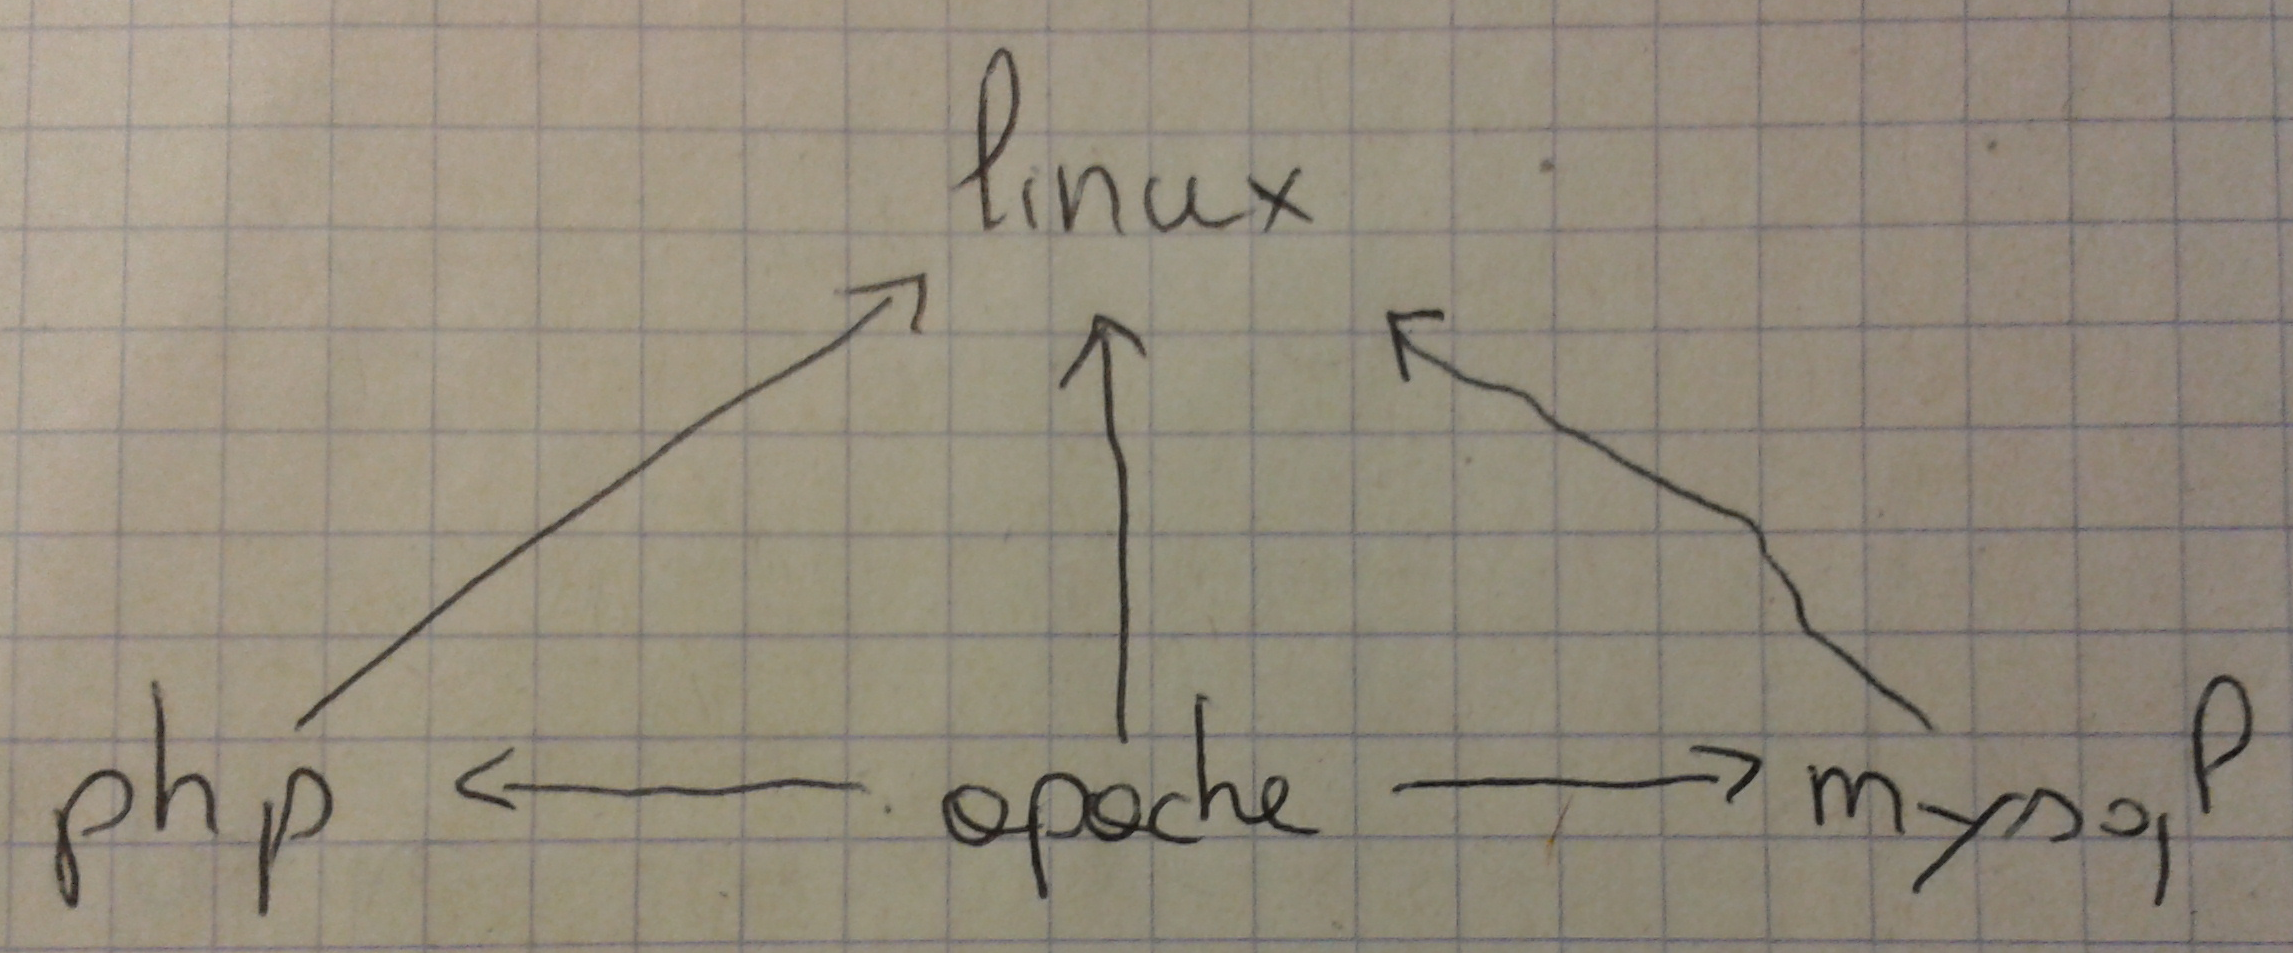
\includegraphics[width=0.6\textwidth]{images/lamp_dep.png}
    \caption{Grafische voorstelling van de afhankelijkheden binnen een LAMP-stack}
    \label{fig:lamp_dep}
    \end{center}
\end{figure}
Als deze afhankelijkheden niet gespecifi\"eerd worden in het model kan de CMS er ook geen rekening mee houden.
Het kan dus dat de tool het model in een foute volgorde uitrolt: eerst de webserver, dan php en uiteindelijk de database.
De webserver zal bij het opstarten proberen te verbinden met de database, maar deze is nog niet online.
In de tijd tussen het opstarten van de webserver en de installatie van PHP zal ze ook geen dynamische webpagina's kunnen tonen.
Een op het eerste zicht succesvolle deployment run kan dus leiden tot een configuratie die niet volledig werkt.

In vergelijking met de beginsituatie is de toestand van de configuratie na de ene run wel al minder afwijkend van de gewenste situatie:
de verschillende pakketten, services en configuratiebestanden zijn al aanwezig.
Tijdens de volgende deployment run zal de Apache service herstart worden en dan zal ze wel kunnen connecteren met de database.

CMS zal nooit aanpassingen maken die zorgen voor een configuratie die verder afwijkt van het model dan voorheen.
Na een paar iteraties zal uiteindelijk altijd de gewenste configuratie bereikt worden. 
Grafisch wordt dit voorgesteld op figuur \ref{fig:convergentie}.
Het aantal iteraties is afhankelijk van de hoeveelheid afhankelijkheden die bestaan maar niet aanwezig zijn in het model.

\begin{figure}[h]
    \begin{center}
    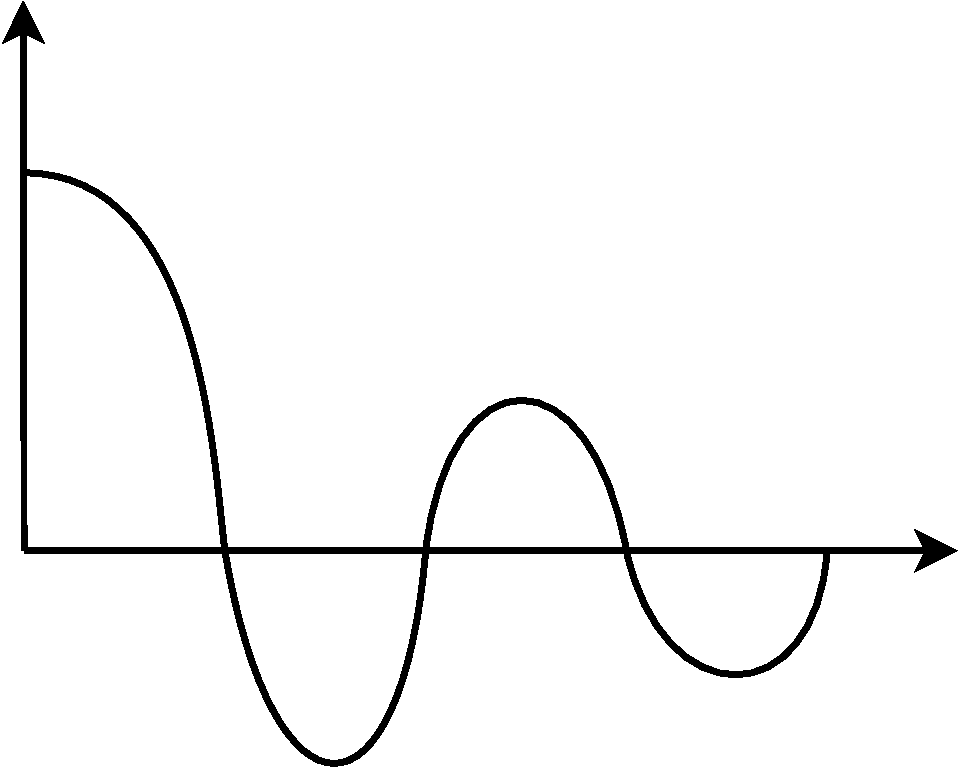
\includegraphics[width=0.6\textwidth]{images/convergentie.png}
    \caption{Grafische voorstelling van de convergentie na een reeks deployment runs.}
    \label{fig:convergentie}
    \end{center}
\end{figure}

%CMS laat vaak toe om logisch samenhorende basisobjecten te verzamelen en   
Databases en webserver zijn abstracties die bestaan uit een verzameling basisobjecten zoals bestanden, pakketten en services.
Tussen deze objecten bestaan er natuurlijk ook afhankelijkheden, bijvoorbeel tussen een bestand en de map waarin het staat:
als de CMS eerst probeert het bestand te cree\"eren en dan pas de map zal de deployment run slechts gedeeltelijk slagen want een bestand kan niet bestaan zonder zijn parent folder.
\begin{figure}[h]
    \begin{center}
    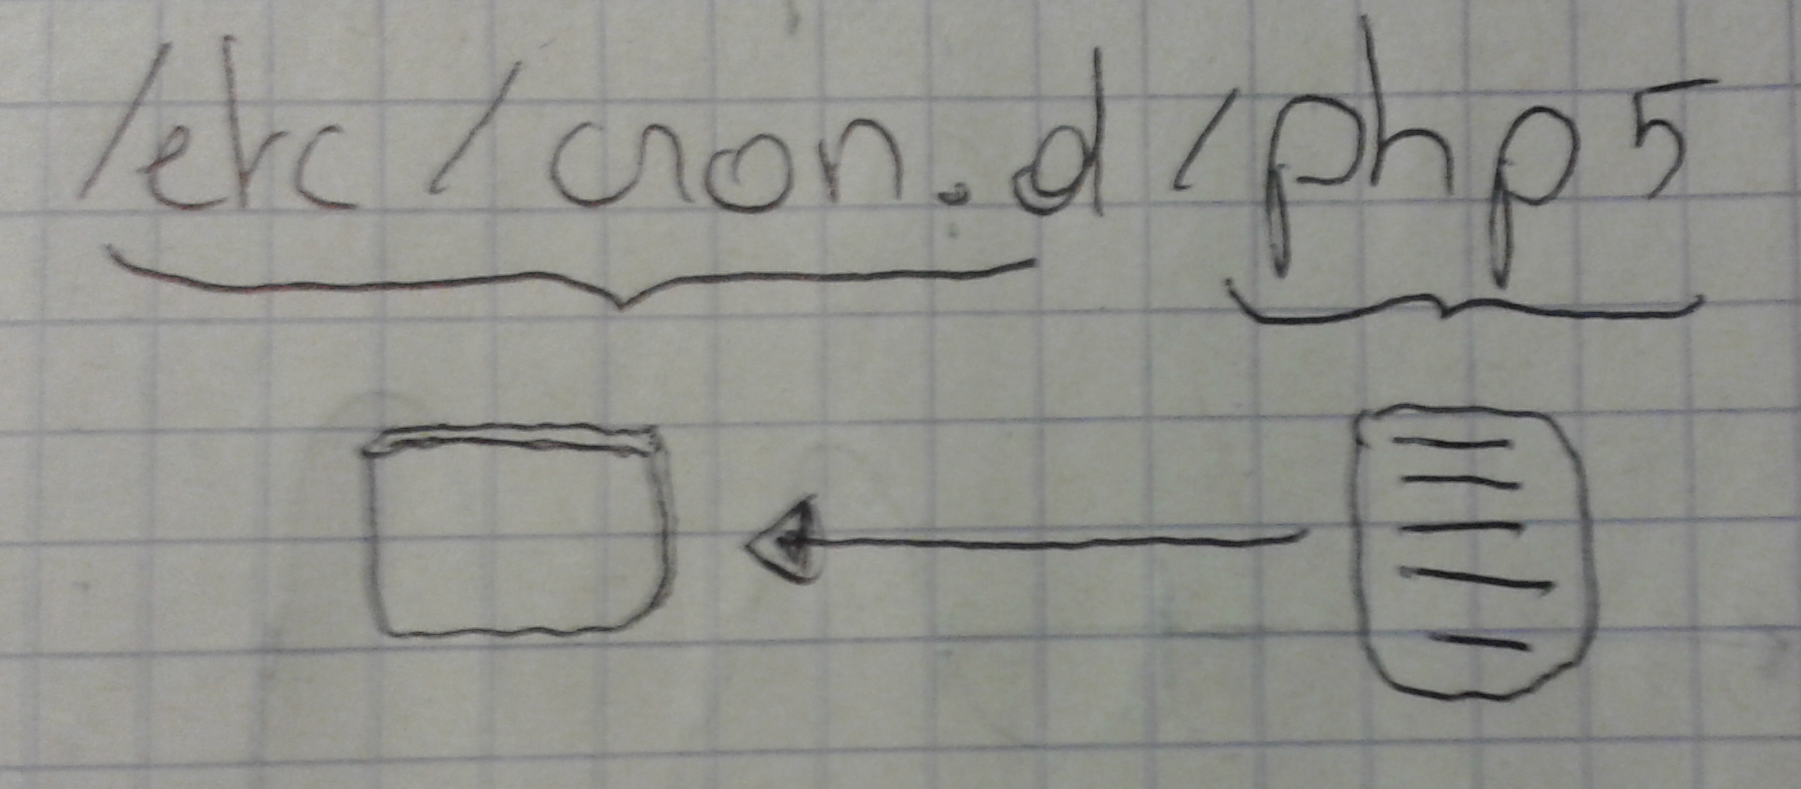
\includegraphics[width=0.6\textwidth]{images/file_dir_dep.png}
    \caption{Grafische voorstelling van de afhankelijkheid tussen een bestand en zijn parent folder}
    \label{fig:file_dir_dep}
    \end{center}
\end{figure}
In vergelijking met het voorbeeld van de LAMP-stack zal de gebruiker direct na het uitrollen al zien dat er iets foutgaat.
De CMS zal namelijk tonen dat sommige resources niet konden aangemaakt worden.
Dit in tegenstelling tot het voorbeeld van de LAMP-stack waarin alles succesvol ge\"installeerd werd. 
Daar zal de gebruiker pas kunnen zien dat er iets fout is als hij de logs van de Apache service bekijkt, of probeert een site te bezoeken.

We kunnen het onderscheid maken tussen twee situaties: vereisten en afhankelijkheden.
In het geval van het bestand en de map is er sprake van een vereiste die niet voldaan is: de map \emph{moet} bestaan v\'o\'or het aanmaken van het bestand of deze wordt niet aangemaakt.
In het geval van de LAMP-stack houdt de CMS geen rekening met de afhankelijkheid tussen de webserver en de databaseserver.
Alle resources worden foutloos aangemaakt maar toch werkt de uiteindelijke configuratie niet omdat een foute volgorde werd gehanteerd.

\todo{Belang: correct gebeuren is van groot belang}

%%%%%%%%%%%%%%%%%%%%%%%%%%%%%%%%%%%%%%%%%%%%%%%%%%%%%
%          Dependencies met huidige tools           %
%%%%%%%%%%%%%%%%%%%%%%%%%%%%%%%%%%%%%%%%%%%%%%%%%%%%%
De huidige CMS laten toe om op het niveau van bestanden, packages en services afhankelijkheden te specifi\"eren.
Bij het uitrollen van een model wordt dan een volgorde opgelegd waarmee de verschillende objecten verwerkt worden.

De tools die momenteel beschikbaar zijn compileren tijdens de deployment voor elke machine hun deel van het model.
Elke machine krijgt dus informatie over wat hijzelf doet maar kan geen rekening houden met wat er op andere machines gebeurt.
Afhankelijkheden binnen \'e\'en machine verwerken is dus geen probleem maar afhankelijkheden tussen verschillende machines zijn niet mogelijk. \todo{Vermelden van workarounds}
De tools die momenteel beschikbaar zijn kunnen dus het hierboven vermelde probleem van een webserver en een database niet oplossen.
%%%%%%%%%%%%%%%%%%%%%%%%%%%%%%%%%%%%%%%%%%%%%%%%%%%%%
%          Dependencies met IMP                     %
%%%%%%%%%%%%%%%%%%%%%%%%%%%%%%%%%%%%%%%%%%%%%%%%%%%%%
IMP (Infrastructure Management Platform) is een nieuwe tool die momenteel nog in ontwikkeling is.
Een andere aanpak tijdens het deployen van een model laat toe afhankelijkheden tussen hoog-niveau objecten te specifi\"eren:
in tegenstelling tot de vorige tools krijgt elke machine het volledige model ter beschikking en niet alleen zijn eigen deel.
Dit laat de machines toe om rekening te houden met afhankelijkheden tussen eigen objecten en die op een andere machine.

%%%%%%%%%%%%%%%%%%%%%%%%%%%%%%%%%%%%%%%%%%%%%%%%%%%%%
%          Probleem/doelstelling                    %
%%%%%%%%%%%%%%%%%%%%%%%%%%%%%%%%%%%%%%%%%%%%%%%%%%%%%
De doelstelling van deze thesis is een effici\"ente manier vinden om een configuratiemodel uit te rollen.
Effici\"ent slaat hier vooral op het vermijden van extra deployment runs door rekening te houden met al dan niet impliciete afhankelijkheden.

%%%%%%%%%%%%%%%%%%%%%%%%%%%%%%%%%%%%%%%%%%%%%%%%%%%%%
%          Kort: hoe oplossing + resultaten         %
%%%%%%%%%%%%%%%%%%%%%%%%%%%%%%%%%%%%%%%%%%%%%%%%%%%%%
